\documentclass[twoside]{book}

% Packages required by doxygen
\usepackage{fixltx2e}
\usepackage{calc}
\usepackage{doxygen}
\usepackage[export]{adjustbox} % also loads graphicx
\usepackage{graphicx}
\usepackage[utf8]{inputenc}
\usepackage{makeidx}
\usepackage{multicol}
\usepackage{multirow}
\PassOptionsToPackage{warn}{textcomp}
\usepackage{textcomp}
\usepackage[nointegrals]{wasysym}
\usepackage[table]{xcolor}

% Font selection
\usepackage[T1]{fontenc}
\usepackage[scaled=.90]{helvet}
\usepackage{courier}
\usepackage{amssymb}
\usepackage{sectsty}
\renewcommand{\familydefault}{\sfdefault}
\allsectionsfont{%
  \fontseries{bc}\selectfont%
  \color{darkgray}%
}
\renewcommand{\DoxyLabelFont}{%
  \fontseries{bc}\selectfont%
  \color{darkgray}%
}
\newcommand{\+}{\discretionary{\mbox{\scriptsize$\hookleftarrow$}}{}{}}

% Page & text layout
\usepackage{geometry}
\geometry{%
  a4paper,%
  top=2.5cm,%
  bottom=2.5cm,%
  left=2.5cm,%
  right=2.5cm%
}
\tolerance=750
\hfuzz=15pt
\hbadness=750
\setlength{\emergencystretch}{15pt}
\setlength{\parindent}{0cm}
\setlength{\parskip}{3ex plus 2ex minus 2ex}
\makeatletter
\renewcommand{\paragraph}{%
  \@startsection{paragraph}{4}{0ex}{-1.0ex}{1.0ex}{%
    \normalfont\normalsize\bfseries\SS@parafont%
  }%
}
\renewcommand{\subparagraph}{%
  \@startsection{subparagraph}{5}{0ex}{-1.0ex}{1.0ex}{%
    \normalfont\normalsize\bfseries\SS@subparafont%
  }%
}
\makeatother

% Headers & footers
\usepackage{fancyhdr}
\pagestyle{fancyplain}
\fancyhead[LE]{\fancyplain{}{\bfseries\thepage}}
\fancyhead[CE]{\fancyplain{}{}}
\fancyhead[RE]{\fancyplain{}{\bfseries\leftmark}}
\fancyhead[LO]{\fancyplain{}{\bfseries\rightmark}}
\fancyhead[CO]{\fancyplain{}{}}
\fancyhead[RO]{\fancyplain{}{\bfseries\thepage}}
\fancyfoot[LE]{\fancyplain{}{}}
\fancyfoot[CE]{\fancyplain{}{}}
\fancyfoot[RE]{\fancyplain{}{\bfseries\scriptsize Generated by Doxygen }}
\fancyfoot[LO]{\fancyplain{}{\bfseries\scriptsize Generated by Doxygen }}
\fancyfoot[CO]{\fancyplain{}{}}
\fancyfoot[RO]{\fancyplain{}{}}
\renewcommand{\footrulewidth}{0.4pt}
\renewcommand{\chaptermark}[1]{%
  \markboth{#1}{}%
}
\renewcommand{\sectionmark}[1]{%
  \markright{\thesection\ #1}%
}

% Indices & bibliography
\usepackage{natbib}
\usepackage[titles]{tocloft}
\setcounter{tocdepth}{3}
\setcounter{secnumdepth}{5}
\makeindex

% Hyperlinks (required, but should be loaded last)
\usepackage{ifpdf}
\ifpdf
  \usepackage[pdftex,pagebackref=true]{hyperref}
\else
  \usepackage[ps2pdf,pagebackref=true]{hyperref}
\fi
\hypersetup{%
  colorlinks=true,%
  linkcolor=blue,%
  citecolor=blue,%
  unicode%
}

% Custom commands
\newcommand{\clearemptydoublepage}{%
  \newpage{\pagestyle{empty}\cleardoublepage}%
}

\usepackage{caption}
\captionsetup{labelsep=space,justification=centering,font={bf},singlelinecheck=off,skip=4pt,position=top}

%===== C O N T E N T S =====

\begin{document}

% Titlepage & ToC
\hypersetup{pageanchor=false,
             bookmarksnumbered=true,
             pdfencoding=unicode
            }
\pagenumbering{alph}
\begin{titlepage}
\vspace*{7cm}
\begin{center}%
{\Large S\+CF }\\
\vspace*{1cm}
{\large Generated by Doxygen 1.8.13}\\
\end{center}
\end{titlepage}
\clearemptydoublepage
\pagenumbering{roman}
\tableofcontents
\clearemptydoublepage
\pagenumbering{arabic}
\hypersetup{pageanchor=true}

%--- Begin generated contents ---
\chapter{Class Index}
\section{Class List}
Here are the classes, structs, unions and interfaces with brief descriptions\+:\begin{DoxyCompactList}
\item\contentsline{section}{\hyperlink{structbfn}{bfn} }{\pageref{structbfn}}{}
\item\contentsline{section}{\hyperlink{structsystem}{system} }{\pageref{structsystem}}{}
\end{DoxyCompactList}

\chapter{File Index}
\section{File List}
Here is a list of all documented files with brief descriptions\+:\begin{DoxyCompactList}
\item\contentsline{section}{/home/abdullah/\+Code/\+C/\+S\+C\+F/include/\hyperlink{basis_8h}{basis.\+h} \\*Header file describing the basis function data structure }{\pageref{basis_8h}}{}
\item\contentsline{section}{/home/abdullah/\+Code/\+C/\+S\+C\+F/include/{\bfseries masses.\+h} }{\pageref{masses_8h}}{}
\item\contentsline{section}{/home/abdullah/\+Code/\+C/\+S\+C\+F/include/{\bfseries system.\+h} }{\pageref{system_8h}}{}
\item\contentsline{section}{/home/abdullah/\+Code/\+C/\+S\+C\+F/include/\hyperlink{THO_8h}{T\+H\+O.\+h} \\*A Documented file }{\pageref{THO_8h}}{}
\item\contentsline{section}{/home/abdullah/\+Code/\+C/\+S\+C\+F/include/{\bfseries utils.\+h} }{\pageref{utils_8h}}{}
\end{DoxyCompactList}

\chapter{Class Documentation}
\hypertarget{structbfn}{}\section{bfn Struct Reference}
\label{structbfn}\index{bfn@{bfn}}
\subsection*{Public Attributes}
\begin{DoxyCompactItemize}
\item 
int \hyperlink{structbfn_a42a90196a5b97792bd4db565897c404d}{nprimitives}
\item 
\mbox{\Hypertarget{structbfn_aa3bcac7c64f2e27ab084807c5be7a129}\label{structbfn_aa3bcac7c64f2e27ab084807c5be7a129}} 
double {\bfseries exps} \mbox{[}3\mbox{]}
\item 
\mbox{\Hypertarget{structbfn_acbe596061c63dcdc511e8248c3f17cb3}\label{structbfn_acbe596061c63dcdc511e8248c3f17cb3}} 
double {\bfseries coefs} \mbox{[}3\mbox{]}
\item 
\mbox{\Hypertarget{structbfn_afc68d122879040738d39eb51a17a4580}\label{structbfn_afc68d122879040738d39eb51a17a4580}} 
double {\bfseries origin} \mbox{[}3\mbox{]}
\item 
\mbox{\Hypertarget{structbfn_a400e60d202aa7c39fded35cdfdb63167}\label{structbfn_a400e60d202aa7c39fded35cdfdb63167}} 
int {\bfseries shell} \mbox{[}3\mbox{]}
\item 
\mbox{\Hypertarget{structbfn_ab0c241c6146ef903e84c1e5b61dc060b}\label{structbfn_ab0c241c6146ef903e84c1e5b61dc060b}} 
double {\bfseries norm} \mbox{[}3\mbox{]}
\item 
\mbox{\Hypertarget{structbfn_a4da7915dbaf7004dc301f88a40ea2073}\label{structbfn_a4da7915dbaf7004dc301f88a40ea2073}} 
double {\bfseries massno}
\end{DoxyCompactItemize}


\subsection{Member Data Documentation}
\mbox{\Hypertarget{structbfn_a42a90196a5b97792bd4db565897c404d}\label{structbfn_a42a90196a5b97792bd4db565897c404d}} 
\index{bfn@{bfn}!nprimitives@{nprimitives}}
\index{nprimitives@{nprimitives}!bfn@{bfn}}
\subsubsection{\texorpdfstring{nprimitives}{nprimitives}}
{\footnotesize\ttfamily int bfn\+::nprimitives}

The number of primitives in each basisfunction. 

The documentation for this struct was generated from the following file\+:\begin{DoxyCompactItemize}
\item 
/home/abdullah/\+Code/\+C/\+S\+C\+F/include/\hyperlink{basis_8h}{basis.\+h}\end{DoxyCompactItemize}

\hypertarget{structsystem}{}\section{system Struct Reference}
\label{structsystem}\index{system@{system}}


Collaboration diagram for system\+:\nopagebreak
\begin{figure}[H]
\begin{center}
\leavevmode
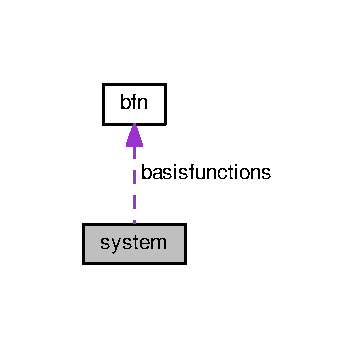
\includegraphics[width=172pt]{structsystem__coll__graph}
\end{center}
\end{figure}
\subsection*{Public Attributes}
\begin{DoxyCompactItemize}
\item 
\mbox{\Hypertarget{structsystem_a050b734bee365115e01985c92259c341}\label{structsystem_a050b734bee365115e01985c92259c341}} 
int {\bfseries natoms}
\item 
\mbox{\Hypertarget{structsystem_af0ef0fc69a0d7507a30b34ad85423107}\label{structsystem_af0ef0fc69a0d7507a30b34ad85423107}} 
int {\bfseries nbfs}
\item 
\mbox{\Hypertarget{structsystem_a3f67573d943d74c49af44e5b58831cc3}\label{structsystem_a3f67573d943d74c49af44e5b58831cc3}} 
\hyperlink{structbfn}{bfn} {\bfseries basisfunctions} \mbox{[}2\mbox{]}
\item 
\mbox{\Hypertarget{structsystem_a09bdd0e4409f90f1bc717c885d4c73ae}\label{structsystem_a09bdd0e4409f90f1bc717c885d4c73ae}} 
double {\bfseries S} \mbox{[}4\mbox{]}
\item 
\mbox{\Hypertarget{structsystem_a5a6a6bc69c5ea5f4766eadfc9bb6d9a0}\label{structsystem_a5a6a6bc69c5ea5f4766eadfc9bb6d9a0}} 
double {\bfseries T} \mbox{[}4\mbox{]}
\item 
\mbox{\Hypertarget{structsystem_aab96dec27f74570c47ba777703c75bce}\label{structsystem_aab96dec27f74570c47ba777703c75bce}} 
double {\bfseries V} \mbox{[}4\mbox{]}
\end{DoxyCompactItemize}


The documentation for this struct was generated from the following file\+:\begin{DoxyCompactItemize}
\item 
/home/abdullah/\+Code/\+C/\+S\+C\+F/include/system.\+h\end{DoxyCompactItemize}

\chapter{File Documentation}
\hypertarget{basis_8h}{}\section{/home/abdullah/\+Code/\+C/\+S\+C\+F/include/basis.h File Reference}
\label{basis_8h}\index{/home/abdullah/\+Code/\+C/\+S\+C\+F/include/basis.\+h@{/home/abdullah/\+Code/\+C/\+S\+C\+F/include/basis.\+h}}


Header file describing the basis function data structure.  


This graph shows which files directly or indirectly include this file\+:\nopagebreak
\begin{figure}[H]
\begin{center}
\leavevmode
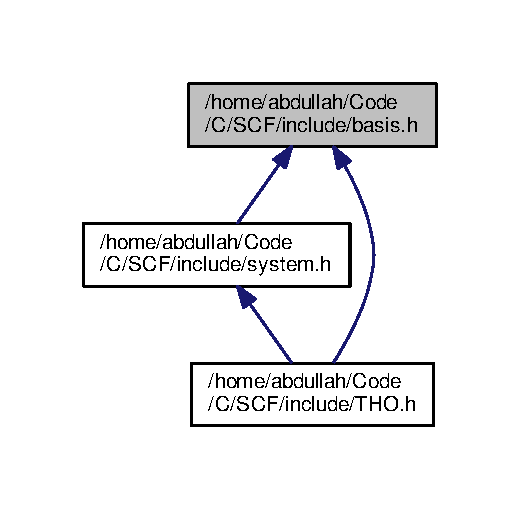
\includegraphics[width=250pt]{basis_8h__dep__incl}
\end{center}
\end{figure}
\subsection*{Classes}
\begin{DoxyCompactItemize}
\item 
struct \hyperlink{structbfn}{bfn}
\end{DoxyCompactItemize}
\subsection*{Typedefs}
\begin{DoxyCompactItemize}
\item 
\mbox{\Hypertarget{basis_8h_af72b9797aefdbee688cfe00652d1be69}\label{basis_8h_af72b9797aefdbee688cfe00652d1be69}} 
typedef struct \hyperlink{structbfn}{bfn} {\bfseries bfn}
\end{DoxyCompactItemize}
\subsection*{Functions}
\begin{DoxyCompactItemize}
\item 
\mbox{\Hypertarget{basis_8h_a718a79a779d96a9b55b1df1ee49e42a4}\label{basis_8h_a718a79a779d96a9b55b1df1ee49e42a4}} 
void {\bfseries bfn\+\_\+set} (\hyperlink{structbfn}{bfn} $\ast$, int, double $\ast$, double $\ast$, int $\ast$, double, double)
\item 
\mbox{\Hypertarget{basis_8h_a87bbfee4e2aeef1bc3ab193e2db90c4c}\label{basis_8h_a87bbfee4e2aeef1bc3ab193e2db90c4c}} 
void {\bfseries normalise} (\hyperlink{structbfn}{bfn} $\ast$)
\end{DoxyCompactItemize}


\subsection{Detailed Description}
Header file describing the basis function data structure. 

\begin{DoxyAuthor}{Author}
Abdullah Ahmad
\end{DoxyAuthor}
Basis function header defining the structure for the bfn struct as well as any member functions. Currently set only for H\+\_\+\{2\} molecule. 
\hypertarget{THO_8h}{}\section{/home/abdullah/\+Code/\+C/\+S\+C\+F/include/\+T\+HO.h File Reference}
\label{THO_8h}\index{/home/abdullah/\+Code/\+C/\+S\+C\+F/include/\+T\+H\+O.\+h@{/home/abdullah/\+Code/\+C/\+S\+C\+F/include/\+T\+H\+O.\+h}}


A Documented file.  


{\ttfamily \#include \char`\"{}basis.\+h\char`\"{}}\newline
{\ttfamily \#include \char`\"{}system.\+h\char`\"{}}\newline
Include dependency graph for T\+H\+O.\+h\+:\nopagebreak
\begin{figure}[H]
\begin{center}
\leavevmode
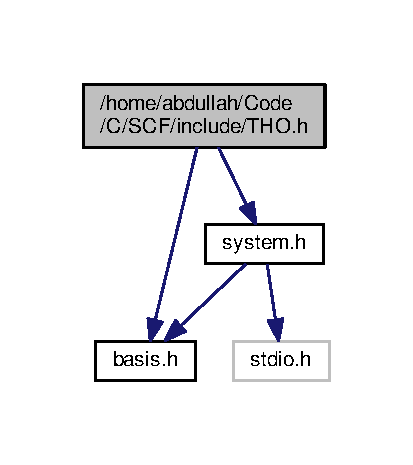
\includegraphics[width=198pt]{THO_8h__incl}
\end{center}
\end{figure}
\subsection*{Functions}
\begin{DoxyCompactItemize}
\item 
\mbox{\Hypertarget{THO_8h_aeec274c7bb08c1ac7a498b67207abfd1}\label{THO_8h_aeec274c7bb08c1ac7a498b67207abfd1}} 
void {\bfseries calculate\+\_\+integral} (\hyperlink{structsystem}{sys} $\ast$)
\item 
\mbox{\Hypertarget{THO_8h_aad250889b35f53a4a0e163a0122c0c57}\label{THO_8h_aad250889b35f53a4a0e163a0122c0c57}} 
double {\bfseries f} (double, double, double, double, double)
\item 
\mbox{\Hypertarget{THO_8h_ab7092e8e82ad913f1e98d6da43e3fab6}\label{THO_8h_ab7092e8e82ad913f1e98d6da43e3fab6}} 
double {\bfseries overlap\+\_\+1d} (int, int, double, double, double)
\item 
\mbox{\Hypertarget{THO_8h_a5ff717eb557df97737508c1ee5498d11}\label{THO_8h_a5ff717eb557df97737508c1ee5498d11}} 
double {\bfseries overlap} (int $\ast$, double $\ast$, double, int $\ast$, double $\ast$, double)
\item 
\mbox{\Hypertarget{THO_8h_a1aa6e63dffea52202c19a3ccc4248eab}\label{THO_8h_a1aa6e63dffea52202c19a3ccc4248eab}} 
double {\bfseries Sab} (\hyperlink{structbfn}{bfn}, \hyperlink{structbfn}{bfn})
\end{DoxyCompactItemize}


\subsection{Detailed Description}
A Documented file. 

Detailed description 
%--- End generated contents ---

% Index
\backmatter
\newpage
\phantomsection
\clearemptydoublepage
\addcontentsline{toc}{chapter}{Index}
\printindex

\end{document}
